 \documentclass[a4paper,12pt]{article}
\usepackage[utf8]{inputenc}
\usepackage{csquotes}
\usepackage[ngerman]{babel}
\usepackage{biblatex}
\usepackage{float}
\usepackage{graphicx}
\usepackage{epstopdf}
\usepackage{subfigure}
\usepackage{graphvizzz}
\usepackage{array}
\usepackage[table]{xcolor}
\usepackage{booktabs}
\usepackage{}
\usepackage{multirow}
\usepackage[format=plain,labelfont=bf,up,justification=centering]{caption}
\setcounter{secnumdepth}{-1} 
\usepackage{hyperref}
\usepackage{nameref}
\usepackage{minted}
\usemintedstyle{friendly}

\bibliography{documentation}
\title{Gesture Remote \\ VLC Remote Control für die Android-Plattform}
\author{Andreas Feldmann \\ Willi Schönborn}
\date{\today}
\begin{document}

\begin{figure}[H]
\centering

\includegraphics[width=0.5\textwidth]{beuth.eps}
\maketitle
\end{figure}

\newpage
\tableofcontents

\newpage
\section*{Projektidee}
Zur Zeit steigt die Nachfrage nach gut bedienbaren Streamingsystemen für den Heimbereich immer weiter an. Dabei wird nicht mehr nur auf die Installation und Wartbarkeit wert gelegt, sondern auch auf die Bedienbarkeit. Und doch können fest installierte Geräte mit Streamingsoftware meist nur über die eingesetzten Peripheriegeräte gesteuert werden. \\
Da sich in den meisten dieser Haushalte auch ein mobiles Endgerät befindet, wäre eine Steuerung der Software über diese Technologie von Vorteil. Dabei spielt vor allem die Art der Steuerung eine wichtige Rolle. Der Benutzer soll nicht nur eine Oberfläche mit entsprechenden Schaltflächen vorfinden, sondern prägnante Gesten, die sich wie bei älteren Geräten vorfindbar, für eine simple Benutzung sorgen. Damit würde, wie bei klassischen TV-Geräten, eine Fernbedienung geschaffen die sich an den einprägsamen Bewegungen (in diesem Fall Gesten) orientiert. \\
Dieses Projekt soll sich mit der Umsetzung einer solchen Remotesteuerung von einem mobilen Endgerät aus, zur Streamingsoftware beschäftigen.

Es gibt frei verfügbare Apps mit ähnlichen Ansätzen. Am interessantesten ist wohl die \textit{Android VLC Remote} App \cite{android-vlc-remote}. Das größte Manko an Apps dieser Art ist, unserer Meinung nach, dass die Möglichkeiten des Smartphones nicht voll ausgereizt werden und damit die Möglichkeiten für eine größere Nutzerzufriedenheit nicht in dem Maße ausgeschöpft werden wie sie könnten.

\newpage
\section*{Konzept}

\subsection*{Gesten}
Alle letztendlich unterstützten Gesten sollen den folgenden Kriterien genügen. Durch die Einhaltung dieser Kriterien versprechen wir uns eine kurze Lernphase und damit extrem kleine Einstiegshürde für Nutzer der App.

\begin{itemize}
	\item \textbf{Erwartungskonform} \\
		Gesten wie Flick, Tap und Scale sind durch bestehende Apps bei vielen Nutzern bereits mental mit entsprechenden Funktionen verknüpft. Diese Erwartungshaltung sollte, sofern möglich, erfüllt werden.
	\item \textbf{Innovativ} \\
		Falls es für bestimmte Funktionen noch keinen De facto-Standard gibt was eine Gestensteuerung betrifft, so sollen neue Gesten gefunden werden, die ggf. so noch nicht genutzt wurden. Wichtig dabei ist jedoch der nächste Punkt.
	\item \textbf{Intuitiv und nachvollziehbar} \\
		Bei neuartigen, ungewohnten oder seltenen Gesten sollte eine Funktion angestoßen werden, die sinnvoll zur entsprechenden Geste passt. Hier sind ggf. kleine A/B-Tests oder eng gefasste Spartakusgruppe-Interviews sinnvoll.
\end{itemize}

Abbildung \ref{fig:gestures} zeigt einige Gesten die ad hoc in Frage kommen sowie mögliche Funktionen, mit denen sie verknüpft werden könnten.

\begin{figure}[H]
\centering
\subfigure[Play/Pause]{
    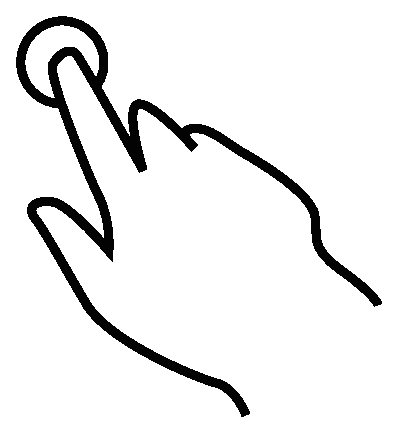
\includegraphics[width=0.2\textwidth]{one_finger_tap_gestureworks.eps}
}
\subfigure[Nächster Titel]{
    \reflectbox{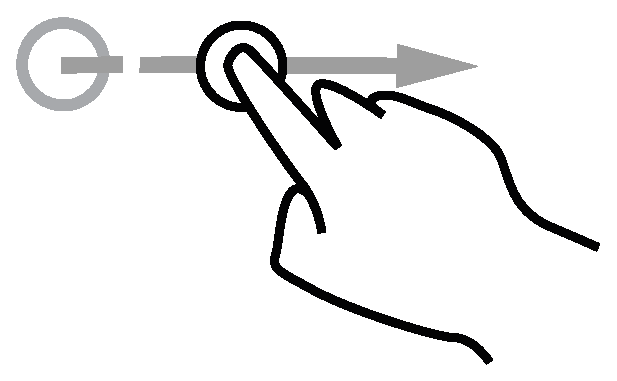
\includegraphics[width=0.35\textwidth]{one_finger_flick_gestureworks.eps}}
}
\subfigure[Vorheriger Titel]{
    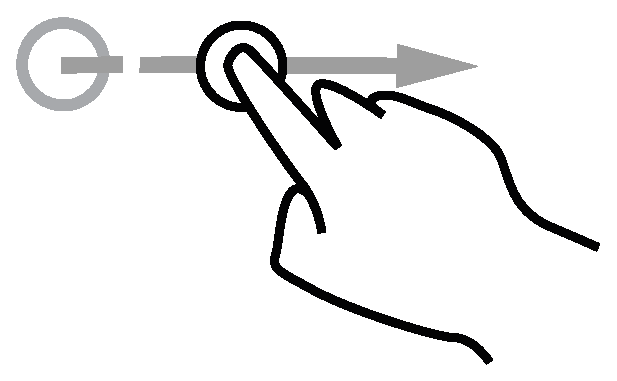
\includegraphics[width=0.35\textwidth]{one_finger_flick_gestureworks.eps}
}
\subfigure[Volume/Seek]{
    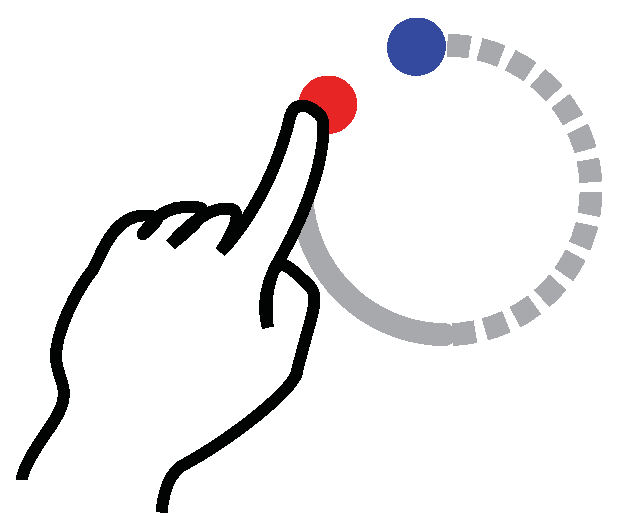
\includegraphics[width=0.3\textwidth]{stroke_shape_circle_gestureworks.eps}
    \label{fig:seek}
}
\subfigure[Vollbild]{
    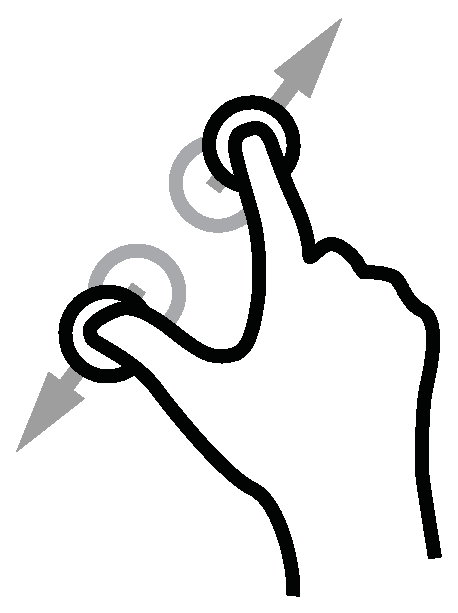
\includegraphics[width=0.2\textwidth]{two_finger_scale_gestureworks.eps}
}
\caption{Gesten}
\label{fig:gestures}
\end{figure}

\newpage
\section{Funktionsumfang}

\newpage
\section{Architektur}

\newpage
\section{Installations- und Bedienungsanleitung}

\newpage
\addcontentsline{toc}{section}{Literatur}
\nocite{*}
\printbibliography

\newpage
\addcontentsline{toc}{section}{Abbildungsverzeichnis}
\listoffigures

\addcontentsline{toc}{section}{Tabellenverzeichnis}
\listoftables

\addcontentsline{toc}{section}{Quellcodeverzeichnis}
\renewcommand\listoflistingscaption{Quellcodeverzeichnis}
\listoflistings

\end{document}

